%
% $Id: ripasso_FIR.tex 14 2014-02-04 22:36:30Z nicb $
%
\svnInfo $Id: ripasso_FIR.tex 14 2014-02-04 22:36:30Z nicb $

\chapter{Un ripasso dei filtri FIR\label{chap:ripasso}}

\section{Trasformata zeta applicata ai filtri FIR\label{sec:zeta fir}}

\subsection{Ritardo e linearit\`a\label{sec:ritardo e linearita}}

Recuperiamo le propriet\`a della trasformata Z e applichiamole ai filtri FIR.

\begin{itemize}

\item filtro FIR:
				
		\begin{equation}
			X(k)\,\raiseto{H}\,Y(k)
		\end{equation}

		La forma generalizzata di un filtro FIR \`e:
  
		\begin{equation}
    	Y(k) = C(1)X(k) + C(2)X(k-1) + ... + C(M)X(k-M+1)
		\end{equation}

\item per via della propriet\`a 2 della trasformata Z (linearit\`a) la trasformata Z di questa somma
     \`e uguale alla somma delle trasformata Z di ogni termine. Per via della propriet\`a
     1, ciascun termine pu\`o essere letto come multiplo della trasformata Z di $X(k)$,
     perch\'e:
 
		 \begin{equation}
			 \begin{array}{r c l}
						 C(1)X(k) & \raiseto{Z} & C(1)X^{*}(z)\\
						 C(2)X(k-1) & \raiseto{Z} & C(2)z^{-1}X^{*}(z)\\
						 C(3)X(k-2) & \raiseto{Z} & C(3)z^{-2}X^{*}(z)\\
						            & \vdots & \\
						 C(M)X(k-M+1) & \raiseto{Z} & C(M)z^{(-M+1)}X^{*}(z)\\
		    \end{array}
		 \end{equation}
 
     quindi:

		 \begin{equation}
						 Y(k)\,\raiseto{Z}\,Y^{*}(z) = [ C(1)+C(2)z^{-1}+C(2)z^{-2}+ \ldots +C(M)z^{-(M+1)} ] X^{*}(z)
		 \end{equation}
 
		 ponendo
 
		 \begin{equation}
			 H(z) = [ C(1)+C(2)z^{-1}+C(2)z^{-2}+ \ldots +C(M)z^{-(M+1)} ]
		 \end{equation}
 
     ossia
 
		 \begin{equation}
						 H(z) = \frac{Y^{*}(z)}{X^{*}(z)}
		 \end{equation}
 
\item quindi: quando $X$ \`e un fasore, anche $Y$ \`e un fasore e il rapporto tra $X$ e
			$Y$ \`e proprio $H(z)$ (quando $z = e^{i\omega}$): quando io metto dentro al filtro un
      segnale sinusoidale ottengo un segnale sinusoidale riscalato

\item ma la faccenda \`e molto pi\`u generale: quando X  \`e  un  qualsiasi
      segnale causale (one-sided), l'uscita di un black box pu\`o  essere
      ottenuta semplicemente moltiplicando la sua trasformata $Z$  per  la
      funzione di trasferimento $H(z)$
 
			\begin{itemize}

			\item facciamo un esempio semplice:
 
				\begin{equation}
	 			\begin{array}{c c c l}
	  			X(k) & = & 0  & \quad per~k~<~0\\
         X(0) & = & 1  &          \\
         X(1) & = & 1  &          \\
				 X(k) & = & 0  & \quad per~k~>~1\\
					\end{array}
			 \end{equation}
 
 \item dalla definizione di trasformata Z ($X^{*}(z) = \sum_0^{N}{X(n)z^{-n}}$), la trasformata di questo segnale \`e:

				 \begin{equation}
								 X^{*}(z) = 1 + z^{-1}
				 \end{equation}
 
 \item ora filtriamolo col solito filtro di media semplicissimo:
 
		 		\begin{equation}
        	 Y(k) = X(k) + X(k-1)
		    \end{equation}
 
 \item la funzione di trasferimento \`e:
 
		 \begin{equation}
						 H(z) = 1 + z^{-1}
		 \end{equation}
 
 \item quindi:
 
		 \begin{equation}
						 Y^{*}(z) = H(z)X^{*}(z) = (1+z^{-1})(1+z^{-1}) = 1 + 2 z^{-1} + z^{-2}
		 \end{equation}

 \item \`e facile fare la trasformata inversa perch\'e ci sono tutte potenze decrescenti
       di zeta, quindi:
 
			 	\begin{equation}
								\begin{array}{c c c l}
           Y(k) & = & 0 & per\,k\,<\,0 \\
           Y(0) & = & 1 & \\
           Y(1) & = & 2 & \\
           Y(2) & = & 1 & \\
           Y(k) & = & 0 & per\,k\,>\,2\\
								\end{array}
		 \end{equation}
 
       si pu\`o verificare la correttezza facendo girare ``a mano'' il filtro

			\end{itemize}
%
%    - dimostrare che la trasformata Z \`e unica per ogni segnale, cio\`e che se due
%      segnali hanno la stessa trasformata Z, allora sono identici
%

\end{itemize}

\subsection*{Esercizi}

\begin{itemize}
 
 \item rifare il filtraggio sopra esposto con il seguente segnale:

				 \begin{equation}
						X(x) = \left\{
						   \begin{array}{c l}
									1 & 0 <= k <= 10 (o\,\,anche\,<=\,5)\\
									0 & altrimenti\\
							 \end{array} \right.
		     \end{equation}
 
       e con le seguenti funzioni di trasferimento:
 
			 	\begin{equation}
					\begin{array}{c c c c c}
	  				H(z) & = & 1 & - & z^{-1}\\
						 H(z) & = & 1 & + & z^{-1}\\
             H(z) & = & ( 1 & - & z^{-1} )^2\\
	      	 \end{array}
	       \end{equation}

\end{itemize}

\section{Una collezione di trasformate zeta notevoli\label{sec:zeta notevoli}}

\subsection{La trasformata zeta pi\`u semplice}

		La trasformata pi\`u semplice \`e quella che prevede campioni  non  zero  per  un
     numero finito di campioni. Per come abbiamo visto l'altra volta, la
     trasformata  $Z$  di  un  segnale  del  genere  \`e  semplicemente  un
     polinomio in $z^{-1}$. P.es.:

		 \begin{equation}
				X(k) = \left\{
					\begin{array}{c c c c}
						0 & k & <= & 0\\
						.5 & k & = & 1\\
						1 & k & = & 2\\
						.5 & k & = & 3\\
						0 & k & > & 3\\
		\end{array} \right.
		 \end{equation}

     Per la definizione di trasformata Z, la trasformata Z di questo segnale \`e

		 \begin{equation}
	   	 X^{*}(z) = .5z^{-1} + z^{-2} + .5z^{-3}
		 \end{equation}

     E la trasformata inversa \`e semplicemente la sequenza dei coefficienti del
     polinomio (== come se fossero ciascuno moltiplicato per 1)

\subsection{Un caso pi\`u interessante}

Un caso pi\`u interessante ha luogo quando il segnale \`e non  zero  per
    un infinito/indefinito numero  di  valori  di  k,  cio\`e  quando  il
    segnale va avanti per sempre. Questo a noi fa comodo per i segnali audio.
    Per noi p.es. sono molto importanti classi di segnali che sono
    esponenziali o sinusoidali di natura, e one-sided.

    Il segnale pi\`u semplice \`e la unit-step function in cui $X(k) = 1$ per $k >= 0$.
		La sua trasformata $z$ \`e:

		 \begin{equation}
						 X^{*}(z) = 1 + z^{-1} + z^{-2} + z^{-3} + \ldots
		 \end{equation}

    Questa \`e una serie geometrica ben conosciuta e sappiamo dall'algebra che
    la sua trasformata $z$ \`e quindi:

		 \begin{equation}
			 X^{*}(z) = \frac{1}{1-z^{-1}}
		 \end{equation}

   La serie geometrica funziona cos\`i: poniamo una serie

		 \begin{equation}
			a + ar + ar^{2} + ar^{3} + ... + ar^{n-1} = \sum_{k=0}^{n-1}{ar^{k}} =  \left\{ a\frac{1-r^{n}}{1 - r} \right\}
		 \end{equation}

   come ci si arriva? poniamo:

		 \begin{equation}
    s = a + ar + ar^{2} + \ldots + ar^{n-1}
		 \end{equation}

   allora 

		 \begin{equation}
    sr = ar + ar^{2} + ar^{3} + ... + ar^{n}
		 \end{equation}

   ma $s - sr = a - ar^{n}$, quindi $s(1 - r) = a(1 - r^{n})$, quindi

		 \begin{equation}
				s = a \frac{1 - r^{n}}{1 - r}
		 \end{equation}

   quando $n$ va all'infinito, \`e necessario che $r < 1$ per far convergere la somma. In questo caso

	 $\sum_{k=0}^{\inf}{ar^{k}}$ diventa $=\frac{a}{1 - r}$ e se $a = 1$, $= \frac{1}{1 - r}$

   quindi 

		 \begin{equation}
			  X^{*}(z) = \frac{1}{1-z^{-1}}
		 \end{equation}

   a patto che $|z^{-1}| < 1$ e dato che $|z^{-1}| = \frac{1}{|z|}$ questo equivale a dire che $|z| > 1$

   Se esaminiamo questo polinomio pi\`u da vicino, e moltiplichiamo num e den
   per $z$, questo diventa:

		 \begin{equation}
						 \frac{z}{z - 1}
		 \end{equation}

   e per $z = 1$, la trasformata zeta diventa infinita. Questo punto si chiama
	 un \emph{polo}. In questo caso quindi la trasformata $z$ ha uno zero per $z = 0$ e
	 un polo per $z = 1$. (un piano con uno zero al centro e un polo sul 1 reale -- cf.Fig.\vref{fig:poli e zeri}).
	 \begin{figure}[Hbtp]
			\begin{center}
				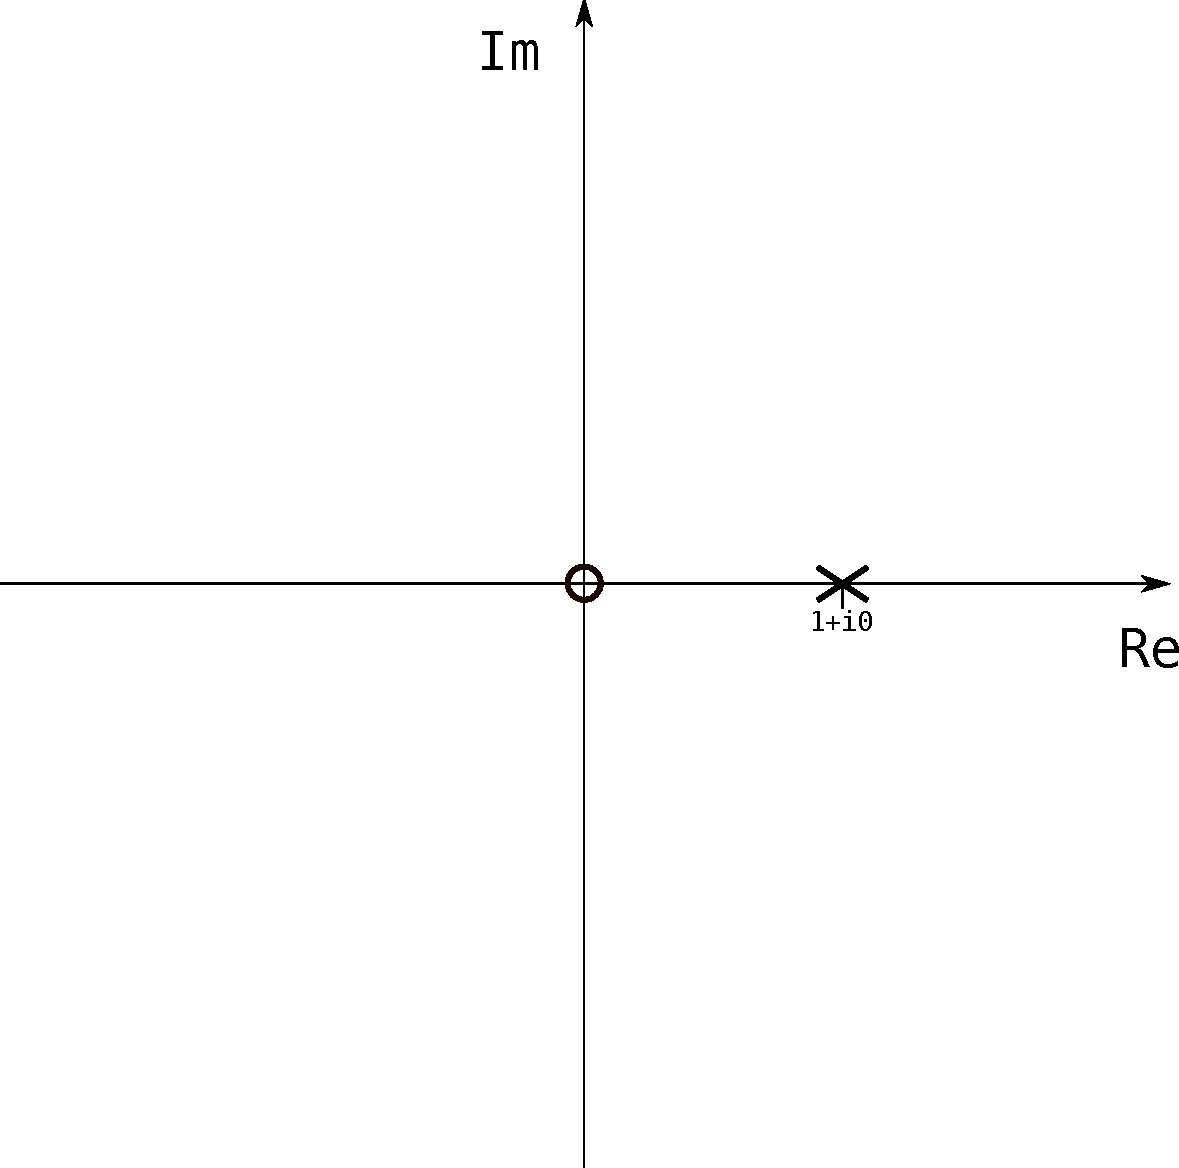
\includegraphics[width=0.35\textwidth]{\imagedir/piano_zeta_un_polo}
				\caption{Poli e zeri del filtro $X^{*}(z) = \frac{1}{1-z^{-1}}$\label{fig:poli e zeri}}
			\end{center}
	 \end{figure}
   Quindi a frequenza zero si sommano tutti gli uni e la somma infinita
   esplode. Possiamo trovare la magnitudine della trasformata $z$ sul cerchio
   unitario e questa si chiama ``contenuto frequenziale'' o \emph{risposta in
	 frequenza} del segnale. Ponendo $z = e^{-i\omega}$

		 \begin{equation}
				X^{*}(z) = \frac{1}{1 - e^{i\omega}}
		 \end{equation}

   la magnitudine (il modulo) \`e quindi:

		 \begin{equation}
				|X^{*}(z)| = \frac{1}{|1 - e^{i\omega}|}
		 \end{equation}


   e se moltiplico entrambi i membri del denominatore per $e^{-iw/2}$ ottengo

		 \begin{equation}
				 |X^{*}(z)| = \frac{1}{|e^{-i\omega/2} - e^{i\omega/2}|}
		 \end{equation}

   e quindi per via della formula di Eulero                 

	   \begin{equation}\label{eqn:infinitefir}
				 |X^{*}(z)| = \frac{1}{2 |sin {\omega/2}|}
		 \end{equation}
	\begin{figure}[htbp]	
		\begin{center}
			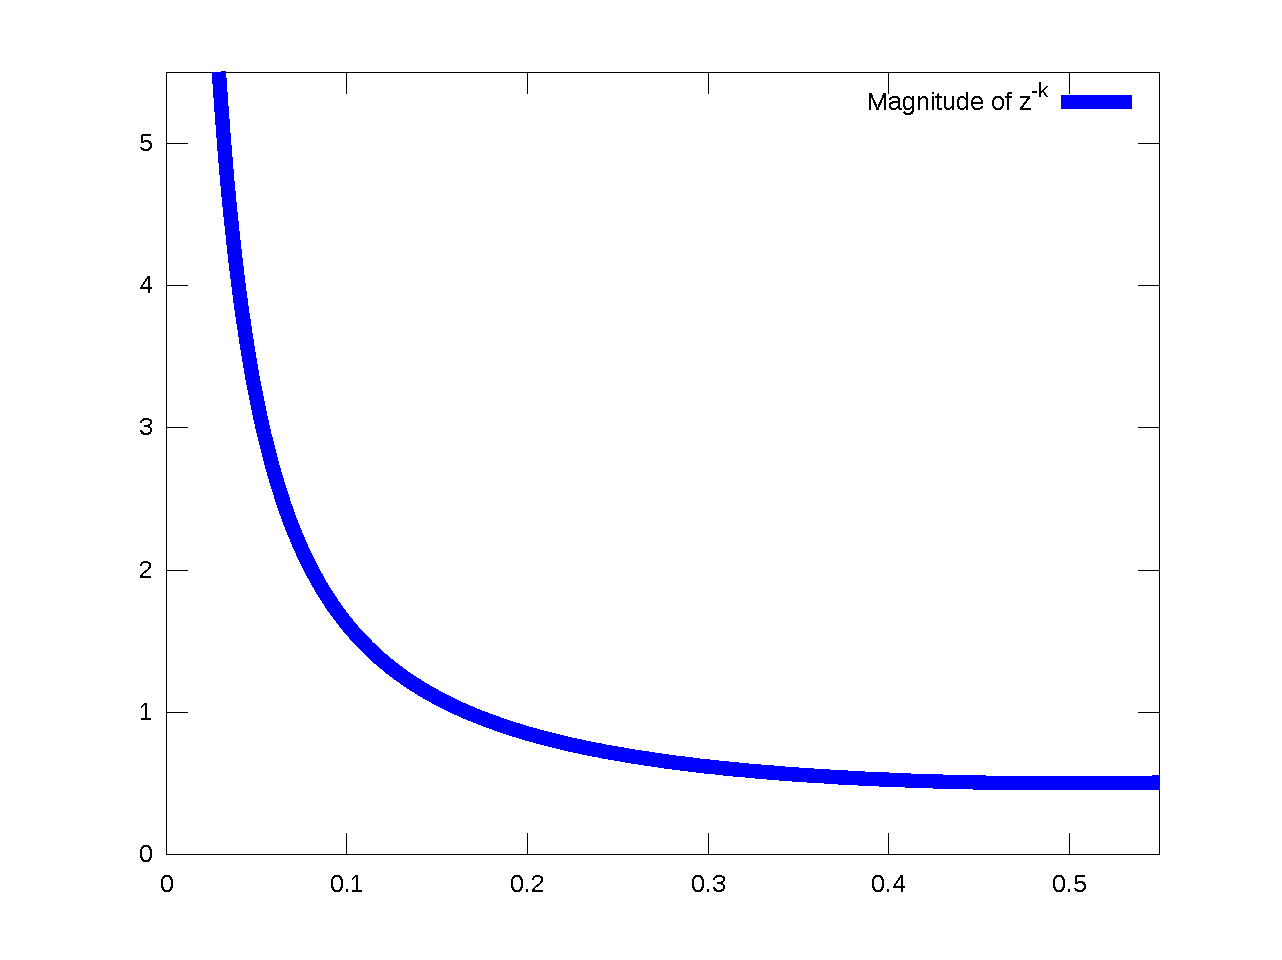
\includegraphics[width=0.4\textwidth]{\plotdir/infinitefir}
			\caption{Magnitudine dell'eq.\ref{eqn:infinitefir} con freq.  normalizzata}
		\end{center}
	\end{figure}
